\section{Desarrollo}




\subsection{Colinealidad}

\begin{figure}[H]
    \centering
    \definecolor{tttttt}{rgb}{0.2,0.2,200}

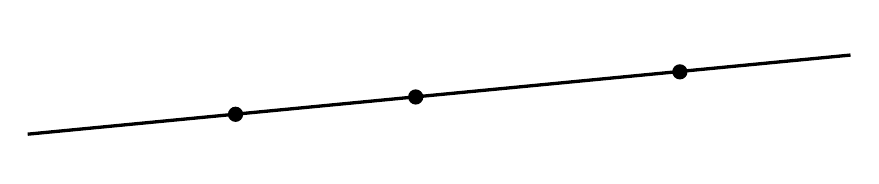
\begin{tikzpicture}[scale = 1.1]
    \clip(-3.6,1.24) rectangle (5.9,2.72);
    \draw [line width=1.2pt,domain=-3.6:5.9] plot(\x,{(--3.82--0.2*\x)/2.08});
    \begin{scriptsize}
        \fill (-1.2,1.72) circle (2.5pt);
        \fill (0.88,1.92) circle (2.5pt);
        \fill (3.93,2.21) circle (2.5pt);
    \end{scriptsize}
\end{tikzpicture}
\end{figure}

Tres puntos son \textbf{colineales} si se encuentran sobre una misma recta.
Dicho esto, presentaremos algunos enfoques que nos ayudarán a probar que tres puntos son colineales al resolver problemas de geometría.

Hay tres formas más comunes de angulear que nos permiten probar que tres puntos $A$, $B$ y $C$ son colineales.

\begin{figure}[H]
    \centering
    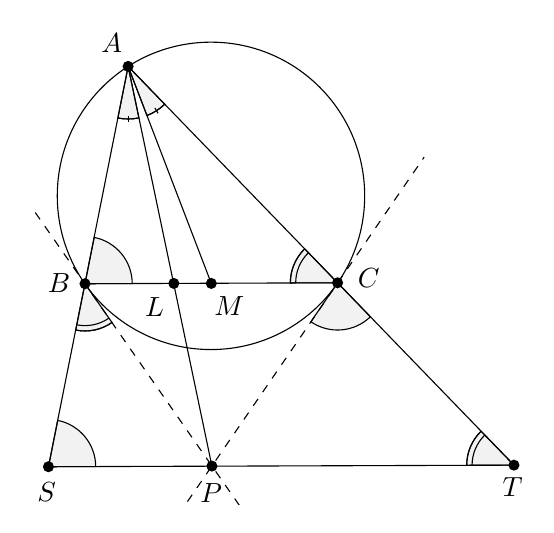
\begin{tikzpicture}[xscale = 0.4, yscale = 0.4]
    \clip(-2.36,-10.08) rectangle (13.47,5.06);
    \draw [shift={(-0.54,-3.07)},fill=black,fill opacity=0.05] (0,0) -- (0.2:1.5) arc (0.2:78.71:1.5) -- cycle;
    \draw [shift={(7.48,-3.04)},fill=black,fill opacity=0.05] (0,0) -- (-124.46:1.5) arc (-124.46:-45.95:1.5) -- cycle;
    \draw [shift={(-1.7,-8.88)},fill=black,fill opacity=0.05] (0,0) -- (0.2:1.5) arc (0.2:78.71:1.5) -- cycle;
    \draw [shift={(-0.54,-3.07)},fill=black,fill opacity=0.05] (0,0) -- (-101.29:1.5) arc (-101.29:-55.14:1.5) -- cycle;
    \draw [shift={(7.48,-3.04)},fill=black,fill opacity=0.05] (0,0) -- (134.05:1.5) arc (134.05:180.2:1.5) -- cycle;
    \draw [shift={(13.08,-8.83)},fill=black,fill opacity=0.05] (0,0) -- (134.05:1.5) arc (134.05:180.2:1.5) -- cycle;
    \draw [shift={(0.83,3.83)},fill=black,fill opacity=0.05] (0,0) -- (-101.29:1.67) arc (-101.29:-78.18:1.67) -- cycle;
    \draw [shift={(0.83,3.83)},fill=black,fill opacity=0.05] (0,0) -- (-69.06:1.67) arc (-69.06:-45.95:1.67) -- cycle;
    \draw(3.46,-0.28) circle (4.88cm);
    \draw (-0.54,-3.07)-- (7.48,-3.04);
    \draw (0.83,3.83)-- (-1.7,-8.88);
    \draw (0.83,3.83)-- (13.08,-8.83);
    \draw (-1.7,-8.88)-- (13.08,-8.83);
    \draw (0.83,3.83)-- (3.49,-8.86);
    \draw (0.83,3.83)-- (3.47,-3.06);
    \draw [dash pattern=on 3pt off 3pt,domain=-2.1176316762214267:13.472829432059696] plot(\x,{(-21.59-8.05*\x)/5.61});
    \draw [dash pattern=on 3pt off 3pt,domain=-2.361745286484902:10.226227746616733] plot(\x,{(--93.93-9.81*\x)/-6.74});
    \draw [shift={(-0.54,-3.07)}] (-101.29:1.5) arc (-101.29:-55.14:1.5);
    \draw [shift={(-0.54,-3.07)}] (-101.29:1.33) arc (-101.29:-55.14:1.33);
    \draw [shift={(7.48,-3.04)}] (134.05:1.5) arc (134.05:180.2:1.5);
    \draw [shift={(7.48,-3.04)}] (134.05:1.33) arc (134.05:180.2:1.33);
    \draw [shift={(13.08,-8.83)}] (134.05:1.5) arc (134.05:180.2:1.5);
    \draw [shift={(13.08,-8.83)}] (134.05:1.33) arc (134.05:180.2:1.33);
    \draw [shift={(0.83,3.83)}] (-101.29:1.67) arc (-101.29:-78.18:1.67);
    \draw(0.84,2.27) -- (0.84,2.07);
    \draw [shift={(0.83,3.83)}] (-69.06:1.67) arc (-69.06:-45.95:1.67);
    \draw(1.68,2.51) -- (1.78,2.34);
    \begin{scriptsize}
        \normalsize
        \fill [color=black] (0.83,3.83) circle (5pt);
        \draw[color=black] (0.31,4.56) node {$A$};
        \fill [color=black] (3.49,-8.86) circle (5pt);
        \draw[color=black] (3.47,-9.7) node {$P$};
        \fill [color=black] (-0.54,-3.07) circle (5pt);
        \draw[color=black] (-1.36,-3.04) node {$B$};
        \fill [color=black] (7.48,-3.04) circle (5pt);
        \draw[color=black] (8.47,-2.88) node {$C$};
        \fill [color=black] (-1.7,-8.88) circle (5pt);
        \draw[color=black] (-1.76,-9.68) node {$S$};
        \fill [color=black] (13.08,-8.83) circle (5pt);
        \draw[color=black] (13.04,-9.54) node {$T$};
        \fill [color=black] (2.28,-3.06) circle (5pt);
        \draw[color=black] (1.67,-3.81) node {$L$};
        \fill [color=black] (3.47,-3.06) circle (5pt);
        \draw[color=black] (4.04,-3.78) node {$M$};
    \end{scriptsize}
\end{tikzpicture}
    \caption{Tres configuraciones de colinealidad.}
\end{figure}

En la primera configuración\footnote{Comenzando de izquierda a derecha.}, necesitaremos dos puntos adicionales que ya son colineales con nuestro punto ``medio'' $B$.
Sean esos puntos $X$ e $Y$.
Si $\angle XBA = \angle YBC$, entonces los puntos $A$, $B$ y $C$ son colineales.

En la segunda configuración, necesitaremos un punto extra $X$ que no esté en la supuesta recta $A - B - C$.
Si $\angle ABX + \angle XBC = 180^\circ$, entonces los puntos $A$, $B$ y $C$ son colineales.

En la tercera configuración, también necesitaremos un punto extra $X$ que no esté en la supuesta recta $A - B - C$.
Si $\angle XAB = \angle XAC$, entonces los puntos $A$, $B$ y $C$ son colineales.




\subsection{Teorema de Menelao}

\begin{section-theorem.tcb}{Teorema de Menelao}{menelaus-theorem}
    Dado un triángulo $ABC$, sean $D$, $E$ y $F$ puntos sobre los lados (posiblemente en sus prolongaciones) $BC$, $CA$ y $AB$, respectivamente.
    Entonces los puntos $D$, $E$ y $F$ son colineales si y sólo si
    \[
        \frac{BD}{DC} \cdot \frac{CE}{EA} \cdot \frac{AF}{FB} = -1.
    \]
\end{section-theorem.tcb}

\begin{figure}[H]
    \centering
    \begin{subfigure}{0.4\textwidth}
    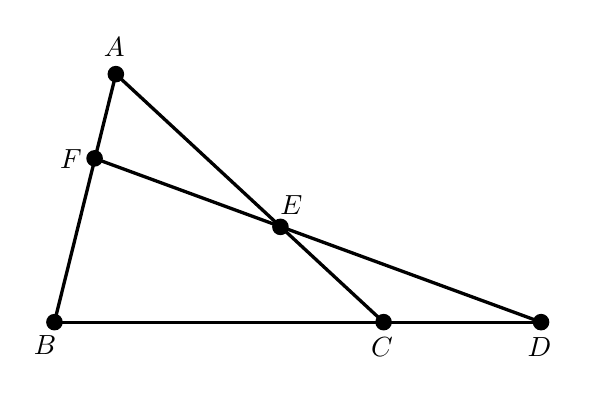
\begin{tikzpicture}[scale = 1]
        \clip(-1.12,1.19) rectangle (5.78,5.6);
        \draw [line width=1.2pt] (0,5.01)-- (3.4,1.86);
        \draw [line width=1.2pt] (-0.78,1.86)-- (0,5.01);
        \draw [line width=1.2pt] (-0.78,1.86)-- (5.4,1.86);
        \draw [line width=1.2pt] (5.4,1.86)-- (-0.27,3.94);
        \begin{scriptsize}
            \normalsize
            \fill [color=black] (0,5.01) circle (3.0pt);
            \draw[color=black] (-0.02,5.36) node {$A$};
            \fill [color=black] (-0.78,1.86) circle (3.0pt);
            \draw[color=black] (-0.9,1.57) node {$B$};
            \fill [color=black] (3.4,1.86) circle (3.0pt);
            \draw[color=black] (3.38,1.55) node {$C$};
            \fill [color=black] (5.4,1.86) circle (3.0pt);
            \draw[color=black] (5.38,1.55) node {$D$};
            \fill [color=black] (2.09,3.07) circle (3.0pt);
            \draw[color=black] (2.23,3.35) node {$E$};
            \fill [color=black] (-0.27,3.94) circle (3.0pt);
            \draw[color=black] (-0.57,3.93) node {$F$};
        \end{scriptsize}
    \end{tikzpicture}
\end{subfigure}
\hspace{0.1\textwidth}
\begin{subfigure}{0.4\textwidth}
    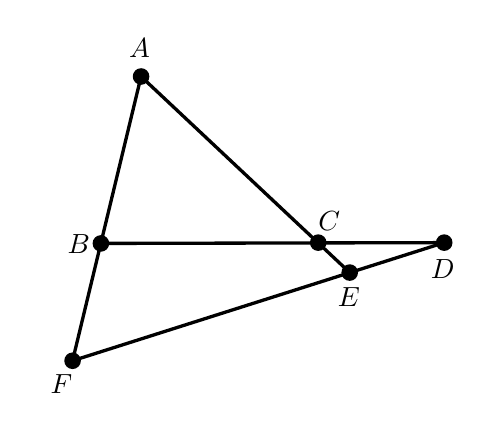
\begin{tikzpicture}[scale = 1]
        \clip(-0.12,0.2) rectangle (5.47,5.01);
        \draw [line width=1.2pt] (1.32,4.39)-- (3.97,1.9);
        \draw [line width=1.2pt] (0.45,0.78)-- (1.32,4.39);
        \draw [line width=1.2pt] (0.45,0.78)-- (5.17,2.28);
        \draw [line width=1.2pt] (5.17,2.28)-- (0.81,2.27);
        \begin{scriptsize}
            \normalsize
            \fill [color=black] (1.32,4.39) circle (3.0pt);
            \draw[color=black] (1.3,4.75) node {$A$};
            \fill [color=black] (0.45,0.78) circle (3.0pt);
            \draw[color=black] (0.31,0.48) node {$F$};
            \fill [color=black] (3.97,1.9) circle (3.0pt);
            \draw[color=black] (3.96,1.59) node {$E$};
            \fill [color=black] (5.17,2.28) circle (3.0pt);
            \draw[color=black] (5.15,1.95) node {$D$};
            \fill [color=black] (3.57,2.28) circle (3.0pt);
            \draw[color=black] (3.71,2.56) node {$C$};
            \fill [color=black] (0.81,2.27) circle (3.0pt);
            \draw[color=black] (0.53,2.26) node {$B$};
        \end{scriptsize}
    \end{tikzpicture}
\end{subfigure}
    \caption{Configuraciones típicas del teorema de Menelao.}
\end{figure}

\begin{proof}
    La demostración se deja como ejercicio al lector.
\end{proof}


\begin{remark.tcb}
    Una manera fácil de recordar cómo escribir esas proporciones\footnote{También funciona para el teorema de \textbf{Ceva}.} es la siguiente.
    Si tenemos el $\triangle XYZ$ y los puntos $M \in XY$, $N \in YZ$ y $P \in ZX$, entonces primero, vamos a escribir los lados de manera cíclica, algo como
    \[
        \frac{X\quad}{\quad Y} \cdot \frac{Y\quad}{\quad Z} \cdot \frac{Z\quad}{\quad X}
    \]
    y después solo tendremos que agregar el punto en el numerador y denominador en la fracción del lado correspondientes, es decir
    \[
        \frac{XM}{MY} \cdot \frac{YN}{NZ} \cdot \frac{ZP}{PX}.
    \]
\end{remark.tcb}


\begin{section-theorem.tcb}{Menelao trigonométrico}{}
    Dado un triángulo $ABC$, sean $D$, $E$ y $F$ puntos sobre los lados (posiblemente en sus prolongaciones) $BC$, $CA$ y $AB$, respectivamente.
    Entonces los puntos $D$, $E$ y $F$ son colineales si y sólo si
    \[
        \frac{\sen(\angle BAD)}{\sen(\angle DAC)} \cdot \frac{\sen(\angle CBE)}{\sen(\angle EBA)} \cdot \frac{\sen(\angle ACF)}{\sen(\angle FCB)} = -1.
    \]
\end{section-theorem.tcb}

\begin{proof}
    La demostración se deja como ejercicio al lector.
\end{proof}

\begin{section-theorem.tcb}{Recta de Gauss}{}
    Sean $L$ y $M$ los puntos medios de las diagonales $AC$ y $BD$ del cuadrilátero $ABCD$.
    Las rectas $AB$ y $CD$ se cortan en $E$, y las rectas $AD$ y $BC$ se cortan en $F$.
    Sea $N$ el punto medio de $EF$.
    Entonces los puntos $L$, $M$ y $N$ colineales.
\end{section-theorem.tcb}

\begin{proof}
    Sean $P$, $Q$ y $R$ los puntos medios de $AE$, $AD$ y $DE$ respectivamente.

    \begin{multicols}{2}

        \begin{figure}[H]
            \centering
            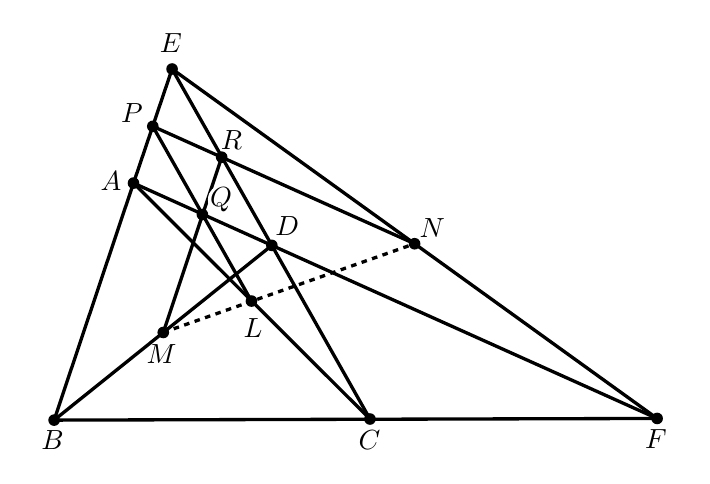
\begin{tikzpicture}[scale = 0.7]
    \clip(-1.74,-0.93) rectangle (10.12,6.84);
    \draw [line width=1.2pt] (-1.26,-0.28)-- (0.18,4.02);
    \draw [line width=1.2pt] (4.47,-0.26)-- (2.69,2.89);
    \draw [line width=1.2pt] (2.69,2.89)-- (0.18,4.02);
    \draw [line width=1.2pt] (-1.26,-0.28)-- (9.68,-0.25);
    \draw [line width=1.2pt] (2.69,2.89)-- (9.68,-0.25);
    \draw [line width=1.2pt] (2.69,2.89)-- (0.88,6.09);
    \draw [line width=1.2pt] (0.18,4.02)-- (0.88,6.09);
    \draw [line width=1.2pt] (0.88,6.09)-- (9.68,-0.25);
    \draw [line width=1.2pt] (-1.26,-0.28)-- (2.69,2.89);
    \draw [line width=1.2pt] (0.18,4.02)-- (4.47,-0.26);
    \draw [line width=1.2pt] (0.53,5.05)-- (2.32,1.88);
    \draw [line width=1.2pt] (1.78,4.49)-- (0.72,1.31);
    \draw [line width=1.2pt] (0.53,5.05)-- (5.28,2.92);
    \draw [line width=1.2pt,dash pattern=on 2pt off 2pt] (0.72,1.31)-- (5.28,2.92);
    \begin{scriptsize}
        \normalsize
        \fill [color=black] (0.18,4.02) circle (3.0pt);
        \draw[color=black] (-0.23,4.06) node {$A$};
        \fill [color=black] (-1.26,-0.28) circle (3.0pt);
        \draw[color=black] (-1.29,-0.65) node {$B$};
        \fill [color=black] (4.47,-0.26) circle (3.0pt);
        \draw[color=black] (4.46,-0.65) node {$C$};
        \fill [color=black] (2.69,2.89) circle (3.0pt);
        \draw[color=black] (2.97,3.24) node {$D$};
        \fill [color=black] (0.88,6.09) circle (3.0pt);
        \draw[color=black] (0.86,6.56) node {$E$};
        \fill [color=black] (9.68,-0.25) circle (3.0pt);
        \draw[color=black] (9.66,-0.63) node {$F$};
        \fill [color=black] (0.72,1.31) circle (3.0pt);
        \draw[color=black] (0.69,0.92) node {$M$};
        \fill [color=black] (2.32,1.88) circle (3.0pt);
        \draw[color=black] (2.35,1.39) node {$L$};
        \fill [color=black] (1.43,3.45) circle (3.0pt);
        \draw[color=black] (1.77,3.72) node[fill = white, rounded corners = 5pt, inner sep=0.8pt] {$Q$};
        \fill [color=black] (0.53,5.05) circle (3.0pt);
        \draw[color=black] (0.15,5.29) node {$P$};
        \fill [color=black] (1.78,4.49) circle (3.0pt);
        \draw[color=black] (1.96,4.81) node[fill = white, rounded corners = 5pt, inner sep=0.8pt] {$R$};
        \fill [color=black] (5.28,2.92) circle (3.0pt);
        \draw[color=black] (5.6,3.2) node {$N$};
    \end{scriptsize}
\end{tikzpicture}
        \end{figure}

        Las rectas $PQ$, $QR$ y $PR$ son bases medias de $ADE$, por lo tanto son las respectivas bases medias de $ACE$, $BDE$ y $AFE$, así que estas pasan por $L$, $M$ y $N$.

        Por semejanza, tenemos que
        \[
            \frac{LQ}{LP} = \frac{CD}{CE},\quad \frac{NP}{NR} = \frac{FA}{FD}\quad \text{y} \quad \frac{MR}{MQ} = \frac{BE}{BA}.
        \]
        Al multiplicar se obtiene
        \[
            \frac{LQ}{LP} \cdot \frac{NP}{NR} \cdot \frac{MR}{MQ} = \frac{CD}{CE} \cdot \frac{FA}{FD} \cdot \frac{BE}{BA}
        \]
    \end{multicols}

    Pero este producto es igual a 1, ya que se cumple el~\refTheorem{\ref{t:menelaus-theorem}} para el triángulo $ADE$ con respecto a la transversal $B-C-F$.
    Se concluye entonces que $L$, $M$ y $N$ son colineales.
\end{proof}




\subsection{Teorema de Pappus}

\begin{section-theorem.tcb}{Teorema de Pappus}{pappus-theorem}
    Sean $A$, $B$ y $C$ tres puntos colineales (no necesariamente en ese orden) y $D$, $E$ y $F$ otros tres puntos colineales (no necesariamente en ese orden).
    Entonces, los puntos de intersección de las rectas $AE$, $BD$; $AF$, $CD$ y $BF$, $CE$ son colineales.
\end{section-theorem.tcb}

\begin{figure}[H]
    \centering
    \definecolor{qqqqcc}{rgb}{0,0,0.8}
%dash pattern=on 5pt off 2pt
%[fill = white, rounded corners = 5pt, inner sep=0.8pt]
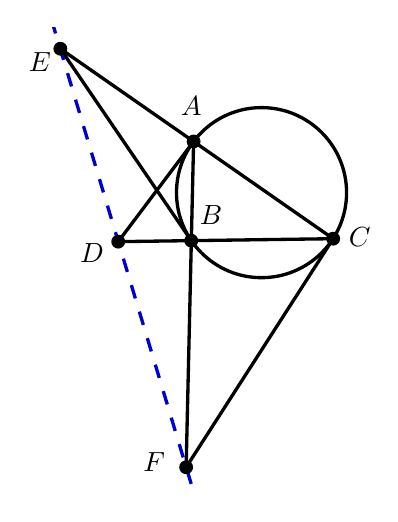
\begin{tikzpicture}[scale = 0.25]
    \clip(-10.02,-12.9) rectangle (7.34,10.77);
    \draw [line width=1.2pt] (1.86,2.39) circle (4.32cm);
    \draw [line width=1.2pt] (-8.36,9.7)-- (5.5,0.05);
    \draw [line width=1.2pt] (-8.36,9.7)-- (-1.71,-0.05);
    \draw [line width=1.2pt] (-5.42,-0.1)-- (5.5,0.05);
    \draw [line width=1.2pt] (-5.42,-0.1)-- (-1.59,4.99);
    \draw [line width=1.2pt] (-1.97,-11.56)-- (5.5,0.05);
    \draw [line width=1.2pt] (-1.97,-11.56)-- (-1.59,4.99);
    \draw [line width=1.2pt,dash pattern=on 5pt off 5pt,color=qqqqcc,domain=-10.02:7.34] plot(\x,{(-115.81-21.26*\x)/6.4});
    \begin{scriptsize}
        \normalsize
        \fill [color=black] (-1.59,4.99) circle (10.0pt);
        \draw[color=black] (-1.71,6.81) node {$A$};
        \fill [color=black] (-1.71,-0.05) circle (10pt);
        \draw[color=black] (-0.7,1.24) node {$B$};
        \fill [color=black] (5.5,0.05) circle (10pt);
        \draw[color=black] (6.85,0.11) node {$C$};
        \fill [color=black] (-8.36,9.7) circle (10pt);
        \draw[color=black] (-9.4,9) node {$E$};
        \fill [color=black] (-5.42,-0.1) circle (10pt);
        \draw[color=black] (-6.75,-0.69) node {$D$};
        \fill [color=black] (-1.97,-11.56) circle (10pt);
        \draw[color=black] (-3.59,-11.3) node {$F$};
    \end{scriptsize}
\end{tikzpicture}
    \caption{Teorema de Pappus.}
    \label{fig:pappus-theorem}
\end{figure}

\begin{multicols}{2}
    Naturalmente, existen muchas configuraciones aparte de las mostradas en la figura \ref{fig:pappus-theorem}, pero esta es la más común.

    Una manera mnemotécnica de indentificar y no olvidar los puntos colineales es la mostrado en la figura~\ref{fig:pappus-mnemonic}.
    \begin{figure}[H]
        \centering
        \includegraphics[width=3.4cm]{images/pappus-points}
        \caption{Mnemotécnia de Pappus.}
        \label{fig:pappus-mnemonic}
    \end{figure}
\end{multicols}

\begin{proof}
    Sean $M = AE \cap BD$, $N = BF \cap CE$ y $P = AF \cap CD$.
    Divideremos la demostración en dos casos, basado en si las rectas $AE$ y $BF$ se intersecan o son paralelas.
    
    \textbf{Caso 1.}
    Si estas se intersecan, sea $AE \cap BF = X$.
    Sea $Y = BF \cap CD$ y $Z = AE \cap CD$.

    \begin{multicols}{2}
        \begin{figure}[H]
            \centering
            \definecolor{qqttzz}{rgb}{0,0.2,0.6}
\definecolor{ccqqqq}{rgb}{0.8,0,0}
\definecolor{qqqqcc}{rgb}{0,0,0.8}
\definecolor{qqqqzz}{rgb}{0,0,0.6}
\definecolor{wwwwww}{rgb}{0.4,0.4,0.4}

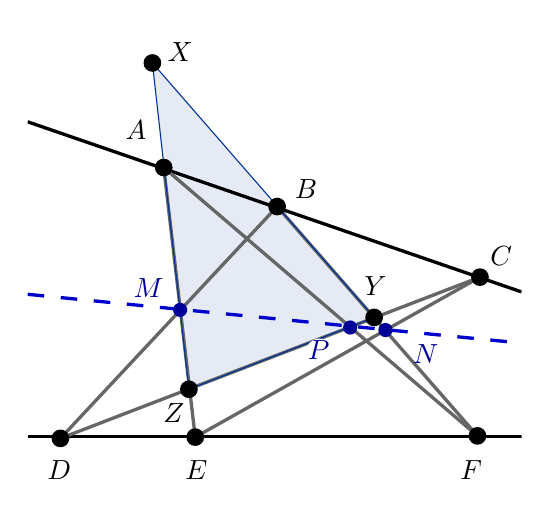
\begin{tikzpicture}[scale = 1.6]
    \clip(-2.86,1.38) rectangle (1.06,5.01);
    \fill[line width=0.4pt,color=qqttzz,fill=qqttzz,fill opacity=0.1] (-1.87,4.73) -- (-1.58,2.14) -- (-0.11,2.71) -- cycle;
    \draw [line width=1.2pt,domain=-2.86:1.06] plot(\x,{(--2.95-0.31*\x)/0.9});
    \draw [line width=1.2pt,domain=-2.86:1.06] plot(\x,{(--1.87-0*\x)/1.06});
    \draw [line width=1.2pt,color=wwwwww] (-1.78,3.9)-- (-1.53,1.76);
    \draw [line width=1.2pt,color=wwwwww] (-1.78,3.9)-- (0.71,1.77);
    \draw [line width=1.2pt,color=wwwwww] (-2.6,1.75)-- (-0.88,3.59);
    \draw [line width=1.2pt,color=wwwwww] (-2.6,1.75)-- (0.73,3.03);
    \draw [line width=1.2pt,color=wwwwww] (-1.53,1.76)-- (0.73,3.03);
    \draw [line width=1.2pt,color=wwwwww] (-0.88,3.59)-- (0.71,1.77);
    \draw [line width=1.2pt,dash pattern=on 6pt off 6pt,color=qqqqcc,domain=-2.86:1.06] plot(\x,{(--4.23-0.16*\x)/1.62});
    \draw [line width=0.4pt,color=qqttzz] (-1.87,4.73)-- (-1.58,2.14);
    \draw [line width=0.4pt,color=qqttzz] (-1.58,2.14)-- (-0.11,2.71);
    \draw [line width=0.4pt,color=qqttzz] (-0.11,2.71)-- (-1.87,4.73);
    \begin{scriptsize}
        \normalsize
        \fill [color=black] (-1.78,3.9) circle (2.0pt);
        \draw[color=black] (-2, 4.2) node {$A$};
        \fill [color=black] (-0.88,3.59) circle (2.0pt);
        \draw[color=black] (-0.65,3.73) node {$B$};
        \fill [color=black] (0.73,3.03) circle (2.0pt);
        \draw[color=black] (0.9,3.2) node {$C$};
        \fill [color=black] (-2.6,1.75) circle (2.0pt);
        \draw[color=black] (-2.61,1.5) node {$D$};
        \fill [color=black] (-1.53,1.76) circle (2.0pt);
        \draw[color=black] (-1.52,1.5) node {$E$};
        \fill [color=black] (0.71,1.77) circle (2.0pt);
        \draw[color=black] (0.66,1.5) node {$F$};
        \fill [color=qqqqzz] (-1.65,2.77) circle (1.6pt);
        \draw[color=qqqqzz] (-1.9,2.94) node {$M$};
        \fill [color=qqqqzz] (-0.3,2.63) circle (1.6pt);
        \draw[color=qqqqzz] (-0.55,2.45) node[fill = white, rounded corners = 5pt, inner sep=0.8pt] {$P$};
        \fill [color=qqqqzz] (-0.02,2.61) circle (1.6pt);
        \draw[color=qqqqzz] (0.30,2.42) node {$N$};
        \fill [color=black] (-1.87,4.73) circle (2.0pt);
        \draw[color=black] (-1.65,4.82) node {$X$};
        \fill [color=black] (-1.58,2.14) circle (2.0pt);
        \draw[color=black] (-1.70,1.95) node {$Z$};
        \fill [color=black] (-0.11,2.71) circle (2.0pt);
        \draw[color=black] (-0.10,2.96) node {$Y$};
    \end{scriptsize}
\end{tikzpicture}
        \end{figure}

        Dado que $M$, $N$ y $P$ son laterales a $\triangle XYZ$, podemos usar el~\refTheorem{\ref{t:menelaus-theorem}} para tratar de probar que son colineales, es decir necesitamos probar que
        \[
            \frac{XN}{NY} \cdot \frac{YP}{PZ} \cdot \frac{ZM}{MX} = 1.
        \]
        Ahora, trataremos de encontrar cada una de estas tres proporciones por medio de la aplicación del~\refTheorem{\ref{t:menelaus-theorem}} con otras rectas que se cruzen con $\triangle XYZ$.
    \end{multicols}

    Para lograr esto, usaremos el~\refTheorem{\ref{t:menelaus-theorem}} tres veces en el $\triangle XYZ$ con las transversales $C - N - E$, $A - P - F$ y $D - M - B$, respectivamente, obtendremos
    \[
        \frac{XN}{NY} \cdot \frac{YC}{CZ} \cdot \frac{ZE}{EX} = 1, \quad \frac{XF}{FY} \cdot \frac{YP}{PZ} \cdot \frac{ZA}{AX} = 1 \quad \text{y} \quad \frac{XB}{BY} \cdot \frac{YD}{DZ} \cdot \frac{ZM}{MX} = 1.
    \]
    Sin embargo, vemos que al multiplicar estos resultados nada se cancela, así que necesitamos hallar otras igualdades tal que usen esos segmentos de recta.

    Rápidamente, vemos que usando el~\refTheorem{\ref{t:menelaus-theorem}} dos veces más en $\triangle XYZ$, pero ahora con las transversales $A - B - C$ y $D - E - F$, obtenemos
    \[
        1 = \frac{XB}{BY} \cdot \frac{YC}{CZ} \cdot \frac{ZA}{AX} \quad \text{y} \quad 1 = \frac{XF}{FY} \cdot \frac{YD}{DZ} \cdot \frac{ZE}{EX}.
    \]
    Multiplicando estas 5 igualdades lado a lado, y viendo que 6 de las fracciones del lado izquierdo de la ecuación se cancelan con cada una las fracciones del lado derecho.
    Quedándonos con lo que queríamos demostrar.

    \textbf{Caso 2.}
    Ahora, veamos que pasa si el punto $X$ no existe, es decir $AE \parallel BF$.
    Observemos que el punto $X$ aparece exactamente dos veces en cada una de las 5 igualdades de arriba, una vez en el numerador y una vez en el denominador.
    Trataremos de encontrar igualdades análogas tal que no usen segmentos que contengan $X$.
    En realidad podemos lograr esto, usando rectas paralelas para encontrar triángulos semejantes.

    \begin{multicols}{2}
        \begin{figure}[H]
            \centering
            \definecolor{ttttff}{rgb}{0.2,0.2,1}
%dash pattern=on 5pt off 2pt
%[fill = white, rounded corners = 4pt, inner sep = 1pt]
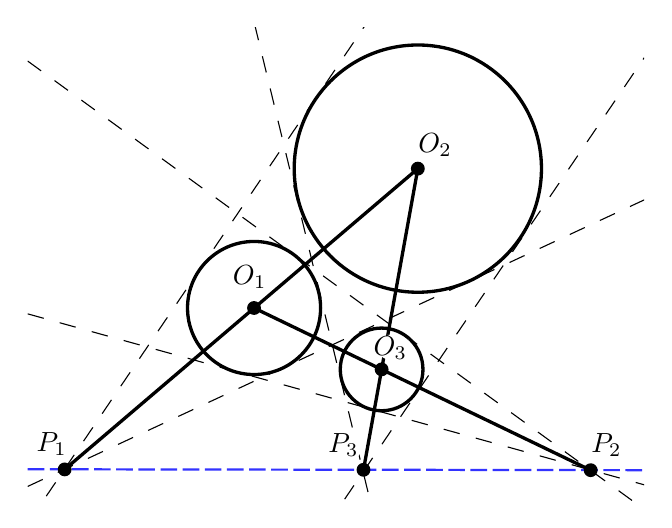
\begin{tikzpicture}[scale = 0.5]
    \clip(4.47,-5.82) rectangle (20.13,6.18);
    \draw [line width=1.2pt] (10.22,-0.94) circle (1.69cm);
    \draw [line width=1.2pt] (13.46,-2.5) circle (1.05cm);
    \draw [line width=1.2pt] (14.38,2.6) circle (3.14cm);
    \draw [line width=1.2pt] (5.41,-5.04)-- (14.38,2.6);
    \draw [line width=1.2pt] (14.38,2.6)-- (13,-5.05);
    \draw [line width=1.2pt] (10.22,-0.94)-- (18.77,-5.06);
    \draw [color = ttttff, dash pattern=on 6pt off 2pt, line width=0.8pt, domain=4.47:20.13] plot(\x,{(-67.19-0.02*\x)/13.36});
    \draw [dash pattern=on 6pt off 6pt,domain=4.47:20.13] plot(\x,{(-41.75--2.57*\x)/5.53});
    \draw [dash pattern=on 6pt off 6pt,domain=4.47:20.13] plot(\x,{(-44.52--5.05*\x)/3.42});
    \draw [dash pattern=on 6pt off 6pt,domain=4.47:20.13] plot(\x,{(-32.25--1.96*\x)/1.33});
    \draw [dash pattern=on 6pt off 6pt,domain=4.47:20.13] plot(\x,{(-27.15--2.31*\x)/-0.56});
    \draw [dash pattern=on 6pt off 6pt,domain=4.47:20.13] plot(\x,{(-40.25--3.41*\x)/-4.69});
    \draw [dash pattern=on 6pt off 6pt,domain=4.47:20.13] plot(\x,{(-0.84--1.55*\x)/-5.59});
    \begin{scriptsize}
        \normalsize
        \fill [color=black] (10.22,-0.94) circle (5pt);
        \draw[color=black] (10.11,-0.15) node[fill = white, rounded corners = 4pt, inner sep = 1pt] {$O_1$};
        \fill [color=black] (14.38,2.6) circle (5pt);
        \draw[color=black] (14.82,3.2) node {$O_2$};
        \fill [color=black] (13.46,-2.5) circle (5pt);
        \draw[color=black] (13.68,-1.95) node[fill = white, rounded corners = 8pt, inner sep = 0.5pt] {$O_3$};
        \fill [color=black] (5.41,-5.04) circle (5pt);
        \draw[color=black] (5.08,-4.4) node {$P_1$};
        \fill [color=black] (18.77,-5.06) circle (5pt);
        \draw[color=black] (19.17,-4.43) node {$P_2$};
        \fill [color=black] (13,-5.05) circle (5pt);
        \draw[color=black] (12.49,-4.43) node[fill = white, rounded corners = 4pt, inner sep = 1pt] {$P_3$};
    \end{scriptsize}
\end{tikzpicture}
        \end{figure}

        Por el criterio \textit{(AA)}, obtenemos que $\triangle CYN \sim \triangle CZE$.
        \[
            \therefore  \quad \frac{CY}{YN} = \frac{CZ}{ZE} \quad \Rightarrow \quad \frac{CY}{YN} \cdot \frac{ZE}{CZ} = 1.
        \]
        Así mismo, obtenemos las siguientes semejanzas $\triangle PYF \sim \triangle PZA$, $\triangle DYB \sim \triangle DZM$, $\triangle YCB \sim \triangle ZCA$ y $\triangle YDF \sim \triangle ZDE$.
        De donde, sacamos igualdades análogas.
    \end{multicols}

    Multiplicando estas igualdades, obtenemos
    \begin{align*}
        &\frac{CY}{YN} \cdot \frac{ZE}{CZ} \cdot \frac{PY}{YF} \cdot \frac{ZA}{PZ} \cdot \frac{DY}{YB} \cdot \frac{ZM}{DZ} \cdot \frac{YB}{YC} \cdot \frac{ZC}{ZA} \cdot \frac{YF}{YD} \cdot \frac{ZD}{ZE} = 1\\[3mm]
        &\therefore \quad \frac{PY}{YN} \cdot \frac{ZM}{PZ} = 1 \quad \Rightarrow \quad \frac{PY}{YN} = \frac{PZ}{ZM}
    \end{align*}
    Como $\angle PYN = \angle PZM$, por \textit{(LAL)} obtenemos que $\triangle PYN \sim \triangle PZM$ y por lo tanto $\angle YPN = \angle ZPM$.
    Ya que $Y - P - Z$ son colineales, por consiguiente $N - P - M$.
\end{proof}




\subsection{Teorema de Desargues}

Consideremos dos triángulos arbitrarios \theTriangle{ABC} y \theTriangle{XYZ}.
Antes de establecer el resultado principal, es necesario proporcionar dos definiciones fundamentales.

\begin{section-definition.tcb}
    \begin{itemize}
        \item Dos triángulos $\triangle ABC$ y $\triangle XYZ$ están en \textit{perspectiva respecto a un \textbf{punto}} (digamos $O$) si las rectas $AX$, $BY$ y $CZ$ son concurrentes.
        \item Dos triángulos $\triangle ABC$ y $\triangle XYZ$ están en \textit{perspectiva respecto a una \textbf{recta}} si los puntos de intersección de los pares de lados correspondientes de ambos triángulos (digamos $P = AB \cap XY$, $Q = CA \cap ZX$ y $R = BC \cap YZ$) son colineales.
    \end{itemize}
\end{section-definition.tcb}

\begin{figure}[H]
    \centering
    \definecolor{ttttff}{rgb}{0.2,0.2,1}
%dash pattern=on 5pt off 2pt
%[fill = white, rounded corners = 5pt, inner sep=0.8pt]
\begin{tikzpicture}[scale = 0.65]
    \clip(8.45,-6.14) rectangle (23.62,4.58);
    \draw [line width=1.2pt] (15.6,-3.7) circle (1.05cm);
    \draw [line width=1.2pt] (10.53,0.69) circle (1.9cm);
    \draw [line width=1.2pt] (19.73,0.87) circle (3.51cm);
    \draw [dash pattern=on 6pt off 6pt,domain=8.45:23.62] plot(\x,{(--25.45-1.98*\x)/0.84});
    \draw [dash pattern=on 6pt off 6pt,domain=8.45:23.62] plot(\x,{(--3.14-0.55*\x)/2.08});
    \draw [dash pattern=on 6pt off 6pt,domain=8.45:23.62] plot(\x,{(-22.13--1.49*\x)/-2.14});
    \draw [dash pattern=on 6pt off 6pt,domain=8.45:23.62] plot(\x,{(--20.12-1.58*\x)/-2.08});
    \draw [dash pattern=on 6pt off 6pt,domain=8.45:23.62] plot(\x,{(-26.17--0.99*\x)/2.19});
    \draw [dash pattern=on 6pt off 6pt,domain=8.45:23.62] plot(\x,{(-35.94--2.28*\x)/0.77});
    \draw [line width=0.8pt, dash pattern=on 6pt off 2pt,color=ttttff,domain=8.45:23.62] plot(\x,{(-88.14--6.4*\x)/-0.09});
    \begin{scriptsize}
        \normalsize
        \fill [color=black] (15.6,-3.7) circle (4pt);
        \draw[color=black] (15.98,-3.18) node {$O_1$};
        \fill [color=black] (19.73,0.87) circle (4pt);
        \draw[color=black] (20.25,1.41) node {$O_2$};
        \fill [color=black] (10.53,0.69) circle (4pt);
        \draw[color=black] (11.01,1.18) node {$O_3$};
        \fill [color=black] (13.84,-5.65) circle (4pt);
        \draw[color=black] (13.28,-5.1) node {$P_1$};
        \fill [color=black] (13.79,-2.14) circle (4pt);
        \draw[color=black] (13.1,-1.41) node {$Q_2$};
        \fill [color=black] (13.76,0.75) circle (4pt);
        \draw[color=black] (13.19,1.76) node {$Q_3$};
    \end{scriptsize}
\end{tikzpicture}
    \caption{Perspectiva de dos triángulos.}
\end{figure}


\begin{section-theorem.tcb}{Teorema de Desargues}{}
    Dos triángulos están en perspectiva con respecto a una recta si y solo si están en perspectiva con respecto un punto.
\end{section-theorem.tcb}

\begin{figure}[H]
    \centering
    
%dash pattern=on 5pt off 2pt
%[fill = white, rounded corners = 4pt, inner sep = 1pt]
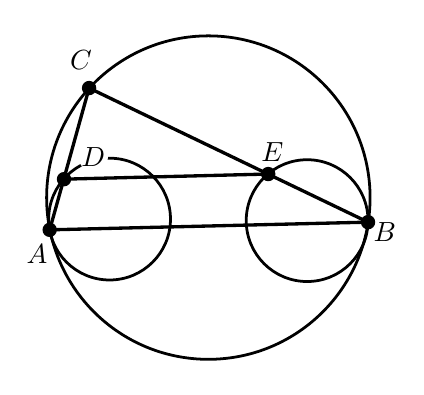
\begin{tikzpicture}[scale = 0.65]
    \clip(12.22,3.3) rectangle (19.42,9.93);
    \draw [line width=1pt] (13.82,6.19) circle (1.19cm);
    \draw [line width=1pt] (17.68,6.16) circle (1.19cm);
    \draw [line width=1pt] (15.75,6.61) circle (3.16cm);
    \draw [line width=1.2pt] (12.65,5.98)-- (18.87,6.13);
    \draw [line width=1.2pt] (18.87,6.13)-- (13.42,8.75);
    \draw [line width=1.2pt] (13.42,8.75)-- (12.65,5.98);
    \draw [line width=1.2pt] (12.93,6.97)-- (16.92,7.07);
    \begin{scriptsize}
        \normalsize
        \fill [color=black] (12.65,5.98) circle (4pt);
        \draw[color=black] (12.4,5.5) node[fill = white, rounded corners = 4pt, inner sep = 1pt] {$A$};
        \fill [color=black] (18.87,6.13) circle (4.0pt);
        \draw[color=black] (19.2,5.93) node {$B$};
        \fill [color=black] (12.93,6.97) circle (4.0pt);
        \draw[color=black] (13.5,7.4) node[fill = white, rounded corners = 4pt, inner sep = 1pt] {$D$};
        \fill [color=black] (16.92,7.07) circle (4.0pt);
        \draw[color=black] (17,7.5) node[fill = white, rounded corners = 4pt, inner sep = 1pt] {$E$};
        \fill [color=black] (13.42,8.75) circle (4.0pt);
        \draw[color=black] (13.26,9.3) node[fill = white, rounded corners = 4pt, inner sep = 1pt] {$C$};
    \end{scriptsize}
\end{tikzpicture}
    \caption{Los triángulos \theTriangle{ABC} y \theTriangle{XYZ} están en perspectiva con $O$ y la recta $PR$.}
\end{figure}

Claramente, al igual que el~\refTheorem{\ref{t:pappus-theorem}}, el teorema de Desargues tiene muchas más configuraciones.

\begin{proof}
    Sean $\triangle ABC$ y $\triangle XYZ$ dos triángulos en perspectiva a un punto, entonces $AX$, $BY$ y $CZ$ son concurrentes con el punto $O$.
    Sea $P = AB \cap XY$, $R = BC \cap YZ$ y $Q = CA \cap ZX$.

    \begin{multicols}{2}
        \begin{figure}[H]
            \centering
            
%dash pattern=on 5pt off 2pt
%[fill = white, rounded corners = 4pt, inner sep = 1pt]
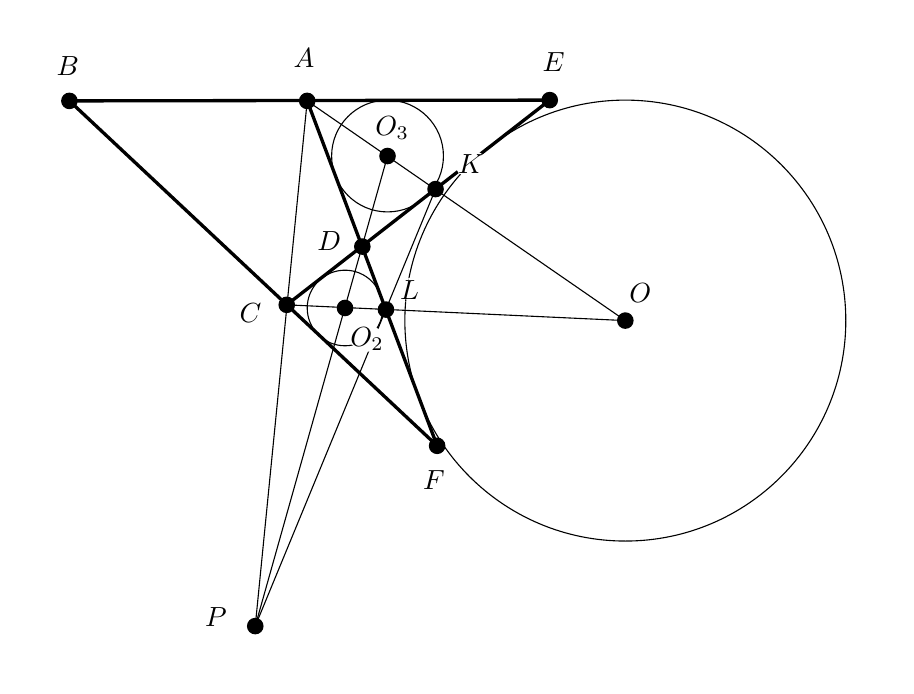
\begin{tikzpicture}[scale = 1]
    \clip(13.07,-0.17) rectangle (23.97,7.93);
    \draw(20.66,4.21) circle (2.8cm);
    \draw(17.1,4.37) circle (0.48cm);
    \draw(17.64,6.3) circle (0.71cm);
    \draw (16.62,7)-- (15.96,0.33);
    \draw (15.96,0.33)-- (17.64,6.3);
    \draw[line width=1.2pt] (18.27,2.62)-- (16.62,7);
    \draw[line width=1.2pt] (19.7,7.01)-- (16.36,4.41);
    \draw (20.66,4.21)-- (16.36,4.41);
    \draw (16.62,7)-- (20.66,4.21);
    \draw (15.96,0.33)-- (18.25,5.88);
    \draw[line width=1.2pt] (13.6,7)-- (19.7,7.01);
    \draw[line width=1.2pt] (13.6,7)-- (18.27,2.62);
    \begin{scriptsize}
        \normalsize
        \fill [color=black] (20.66,4.21) circle (3.0pt);
        \draw[color=black] (20.85,4.56) node {$O$};
        \fill [color=black] (13.6,7) circle (3.0pt);
        \draw[color=black] (13.58,7.44) node {$B$};
        \fill [color=black] (16.62,7) circle (3.0pt);
        \draw[color=black] (16.58,7.54) node {$A$};
        \fill [color=black] (18.27,2.62) circle (3.0pt);
        \draw[color=black] (18.23,2.19) node {$F$};
        \fill [color=black] (19.7,7.01) circle (3.0pt);
        \draw[color=black] (19.75,7.49) node {$E$};
        \fill [color=black] (16.36,4.41) circle (3.0pt);
        \draw[color=black] (15.9,4.3) node {$C$};
        \fill [color=black] (17.32,5.15) circle (3.0pt);
        \draw[color=black] (16.9,5.22) node {$D$};
        \fill [color=black] (17.62,4.35) circle (3.0pt);
        \draw[color=black] (17.92, 4.6) node[fill = white, rounded corners = 6pt, inner sep = 0.8pt] {$L$};
        \fill [color=black] (18.25,5.88) circle (3.0pt);
        \draw[color=black] (18.7,6.2) node[fill = white, rounded corners = 4pt, inner sep = 1pt] {$K$};
        \fill [color=black] (15.96,0.33) circle (3.0pt);
        \draw[color=black] (15.46,0.45) node {$P$};
        \fill [color=black] (17.1,4.37) circle (3pt);
        \draw[color=black] (17.38, 3.98) node[fill = white, rounded corners = 6pt, inner sep = 0.5pt] {$O_2$};
        \fill [color=black] (17.64,6.3) circle (3.0pt);
        \draw[color=black] (17.7,6.65) node[fill = white, rounded corners = 6pt, inner sep = 0.5pt] {$O_3$};
    \end{scriptsize}
\end{tikzpicture}
        \end{figure}

        Aplicando el~\refTheorem{\ref{t:menelaus-theorem}} a los triángulos $\triangle OAB$ con la transversal $P - Y - X$, $\triangle OBC$ con la transversal $R - Z - Y$ y $\triangle OCA$ con la transversal $Q - Z - X$, obtenemos que;
        \begin{align*}
            \frac{OX}{XA} \cdot \frac{AP}{PB} \cdot \frac{BY}{YO} &= 1,\\[1mm]
            \frac{OY}{YB} \cdot \frac{BR}{RC} \cdot \frac{CZ}{ZO} &= 1\quad \text{y}\\[1mm]
            \frac{OZ}{ZC} \cdot \frac{CQ}{QA} \cdot \frac{AX}{XO} &= 1.
        \end{align*}
    \end{multicols}

    Multiplicando estas tres igualdades, llegamos al siguiente resultado
    \[
        \frac{AP}{PB} \cdot \frac{BR}{RC} \cdot \frac{CQ}{QA} = 1,
    \]
    que por el~\refTheorem{\ref{t:menelaus-theorem}} aplicado al triángulo $\triangle ABC$, significa que los puntos $P$, $R$ y $Q$ son colineales, es decir $\triangle ABC$ y $\triangle XYZ$ están en perspectiva con respecto a la recta $PQ$.

    Ahora, probaremos la otra dirección.
    Sean $\triangle ABC$ y $\triangle XYZ$ dos triángulos en perspectiva a un recta, entonces los puntos $P = AB \cap XY$, $Q = CA \cap ZX$ y $R = BC \cap YZ$ son colineales.

    \begin{multicols}{2}
        \begin{figure}[H]
            \centering
            \input{figures/figure-10}
        \end{figure}

        Sean $O = BY \cap CZ$.
        Debemos de probar que $AX$ también pasa por $O$.

        Observemos los triángulos \theTriangle{QCZ} y \theTriangle{PBY}.
        Las rectas $QP$, $CB$ y $ZY$ con concurrentes en $R$, así que los triángulos están en perspectiva con respecto a ese punto.

        Por la dirección del teorema de Desargues que acabamos de demostrar, se deduce que los triángulos deben de estar en perspectiva respecto a una recta.
    \end{multicols}

    Es decir, los puntos $QC \cap PB = A$, $CZ \cap BY = O$ y $ZQ \cap YP = X$ son colineales.
    Con esto, probamos que $AX$ pasa por $O$, luego \theTriangle{ABC} y \theTriangle{XYZ} están en perspectiva respecto al punto $O$.
\end{proof}




\subsection{Agregados culturales y preguntas}

\begin{itemize}
    \item La eficiencia de aplicar el teorema de Menelao puede acelerarse utilizando su versión trigonométrica.
    \item El teorema de Desargues puede servir para transformar una colinealidad en una concurrencia más fácil de trabajar por Ceva, o viceversa, transformando una concurrencia en una colinealidad más fácil de trabajar por Menelao.
    \item ¿Conoces los polígonos degenerados?
    Pues es un polígono en el que algunos de sus vértices coinciden.
    Ejemplos, una recta la podemos considerar tanto como un triángulo degenerado o cuadrilátero degenerado, un pentágono como un héxagono degenerado, etc.
    \item Tanto el teorema de Menelao, Pappus como Desargues tienen su versiones degeneradas, para lo cual se vuelve conveniente considerar rectas paralelas y puntos al infinito.
    En particular la versión degenerada del teorema de Desargues aparece frecuentemente.
\end{itemize}




\section{Ejercicios y Problemas}
Sección de ejercicios y problemas para el autoestudio.
\begin{section-problem}
    Demuestre que las tangentes a la circunferencia circunscrita a un triángulo en los vértices de este, cortan a los lados opuestos de dicho triángulo en tres puntos colineales.
\end{section-problem}

\begin{section-problem}
    Si los lados $AB$, $BC$, $CD$ y $DA$ de un cuadrilátero $ABCD$ son cortados por una transversal en los puntos $A'$, $B'$, $C'$ y $D'$, respectivamente.
    Probar que
    \[
        \dfrac{AA}{A'B} \cdot \dfrac{BB'}{B'C} \cdot \dfrac{CC'}{C'D} \cdot \dfrac{DD'}{D'A} = 1.
    \]
\end{section-problem}

\begin{section-problem}
    Sean $AD$, $BE$ y $CF$ tres cevianas concurrentes en un triángulo \theTriangle{ABC}.
    Se toma un punto $D'$ en $BC$ tal que $BD = CD'$.
    Las paralelas a $BC$ por $E$ y $F$ cortan $AD$ y $AD'$ en $G$ y $H$ respectivamente.
    Prueba que $C$, $G$ y $H$ son colineales.
\end{section-problem}

\begin{section-problem}
    En un paralelogramo $ABCD$ con $\angle B < 90^\circ$, el círculo de diámetro $AC$ corta las rectas $CB$ y $CD$ en $E$ y $F$, respectivamente, y la tangente al círculo por $A$ corto $BD$ en $P$.
    Demuestre que $P$, $F$ y $E$ están alineados.
\end{section-problem}

\begin{section-problem}
    Sea $ABCD$ un cuadrilátero cíclico.
    Las diagonales $AC$ y $BD$ se cortan en $E$, y los lados $AB$ y $CD$ se cortan en $F$.
    Sean $J$ y $K$ los ortocentros de \theTriangle{ADF} y \theTriangle{BCF} respectivamente.
    Demuestre que $J$, $E$ y $K$ están alineados.
\end{section-problem}

\begin{section-problem}
    Sea $ABCD$ un trapecio con $AB$ mayor y paralelo a $CD$.
    Sean $E$ y $F$ puntos en $AB$ y $CD$ respectivamente, tales que $\frac{AE}{EB} = \frac{DF}{FC}$.
    Sean $K$ y $L$ puntos en $EF$ tales que $\angle AKB = \angle DCB$ y $\angle CLD = \angle CBA$.
    Demuestre que $KLCB$ es cíclo.
\end{section-problem}

\begin{section-problem}
    Sea $P$ la intersección de las diagonales $AC$ y $BD$ en el cuadrilátero cíclico $ABCD$.
    Sean $E$, $F$, $G$ y $H$ los pies de las perpendiculares desde $P$ hacía $AB$, $BC$, $CD$ y $DA$, respectivamente.
    Pruebe que las rectas $EH$, $BD$ y $FG$ son concurrentes o son paralelas.
\end{section-problem}
